\documentclass[12pt]{article}
\usepackage[]{algorithm2e}
\usepackage{setspace}
\usepackage[margin=1in]{geometry}
\usepackage{graphicx}
\graphicspath{ {gfx/} }
\usepackage[capitalize]{cleveref}
\usepackage{subfig}
\usepackage{verbatim}
\usepackage{pdfpages}
\usepackage{url}
\usepackage{listings}
\usepackage{ragged2e}

\newcommand{\red}[1]{\textcolor{red}{#1}}

\lstset { language=C++,
	basicstyle=\footnotesize\ttfamily,% basic font setting
	%basicstyle=\scriptsize\ttfamily,% basic font setting
}


%\DeclareGraphicsExtensions{.pdf,.jpg,.png}
\doublespacing
\title{Exploration and Optimization of Tardis: A Novel Cache Coherence Protocol}
\date{}
\begin{document}
	\maketitle
\begin{center}
\textbf{Abstract}
\end{center}

\justify
In a world where data and information are being processed and transferred at an ever-increasing rate, the need for multiple processors has become popular in recent years. With multi-processor machines, computing power is significantly improved, but the problem of sharing memory between cores, or memory coherence, arises. A recently proposed solution that is both simpler and more scalable than the widely used directory coherence, Tardis, uses timestamp counters to logically order memory operations to maintain sequential consistency, as opposed to using physical time. The vanilla Tardis protocol, however, uses long hardware counters for timestamp storage. Additionally, for some applications, Tardis generates a large number of renew requests which consumes the precious network bandwidth. Thus, we propose several optimizations: a timestamp compression scheme to reduce the memory cost of storing timestamps, and several lease predictor protocols to increase efficiency by minimizing the number of renewal requests due to cacheline expiration. The total optimization results are an increase of up to 6\% in throughput and a renew rate reduction from 32\% to 26\%.



\section{Introduction}

\begin{figure}
\begin{center}
  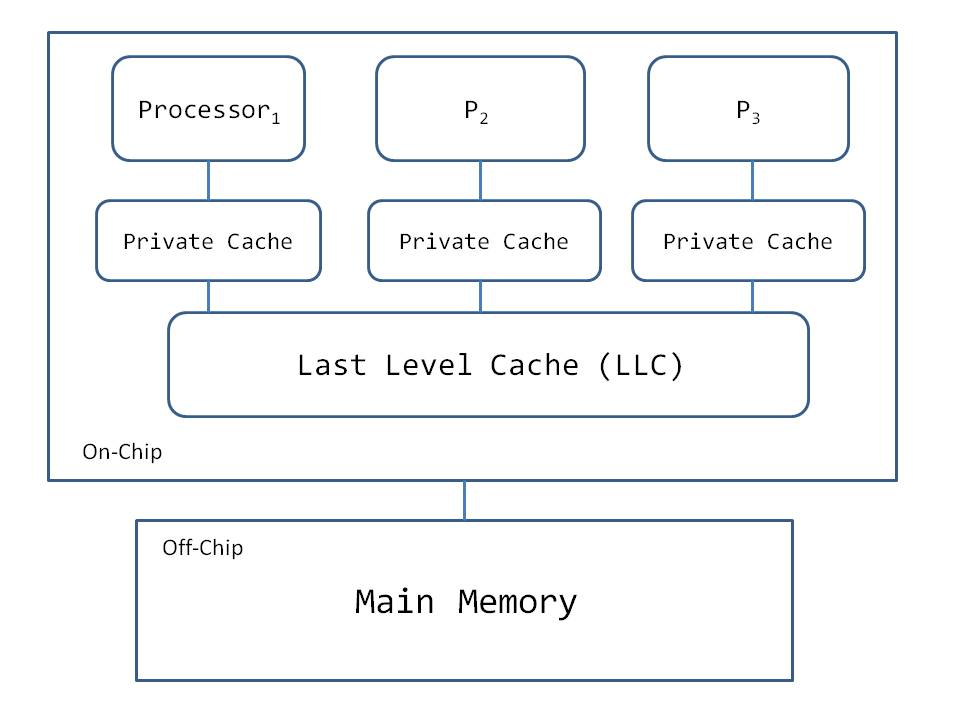
\includegraphics[width=10cm]{distributed_system.JPG}
  \caption{Simple diagram of a shared memory system.}
  \label{fig:distributed}
\end{center}
\end{figure}


In the modern day, there is a continuously increasing demand for 
faster computer processors. Since one of the most effective methods to 
address this is to add multiple cores to a CPU and allowing tasks to 
execute in parallel, the number of cores is increasing 
exponentially~\cite{tilera, xeonphi}. 
% The following statement cannot be right...
% (a certain IBM chip contains 4,000 processor cores [cite?]). 
% 
Multiple cores allow for tasks to be split up and handled 
simultaneously, but accurate and efficient performance requires 
parallelism and exploitation of private cache at each core.  The 
essence of maintaining ``correctness'' is to prevent the use of stale 
data~\cite{lamport1978}, which is old information that is being used 
when it has already been altered by another core. This problem is 
known as memory coherence, and a coherence protocol is necessary to 
facilitate performance and scalability of the system.

Memory coherence is most commonly and traditionally addressed by 
directory based coherence protocols~\cite{censier1978, tang1976}, 
which are relatively intuitive. In such a system a central directory
tracks the coherence between the private caches, or how they are being
owned or shared between cores. Thus, if a core requests private
ownership of a cacheline (the basic unit of data storage), it must
go through the directory so that the lines cached in other cores are 
invalidated accordingly. Since the directory must maintain the sharer 
information for every cacheline, the system requires O(N) storage per 
cacheline if there are N cores.  As N increases, the directory based 
protocol does not scale well.

This problem can be addressed by Tardis~\cite{tardis}, a new coherence 
protocol that is currently in development and has been mathematically 
proven to be correct~\cite{tardis-proof}. Tardis utilizes logical 
timestamps (to be explained in more detail in Background) to enforce 
the global memory order. The protocol only requires O(log N) storage 
per cacheline and is therefore significantly more scalable as well as 
being simpler. However, the major disadvantages of the vanilla Tardis 
protocol is managing very large timestamps and dealing with 
potentially many renewal requests, most of which are unnecessary. 

The goal of this paper is to explore the design space of Tardis and 
optimize the protocol through timestamp compression and renewal 
minimization. We implemented a clever base timestamp + delta scheme to 
reduce the storage overhead of timestamps, designed a livelock 
detection algorithm to prevent several worst-case-scenarios of 
spinning variables, and implemented and analyzed several 
configurations of leasing protocols to reduce the number of renewals. Our total gains improved throughput by up to 6\% and reduced renew rate from 32\% to 26\%.

\section{Background}

Tardis uses logical timestamps to organize shared memory and ensure coherence, which allows it to be simple yet very scalable. By operating with logical time instead of physical time, Tardis is even able to perform actions that seemingly “travel in time,” a phenomenon that will be elaborated upon further on. Henceforth, time will refer to logical time.
To give an analogy, think of a book in the library that two people want to read and then a third wants edit. Intuitively, it would seem that the two readers must first finish reading the book before the third can edit, but Tardis allows all three people to perform their tasks at the same time.  Using arbitrary but realistic numbers, the first person may read the book from logical time 0 to 10, the second person reads from 0 to 20, and the editor “travels in time” and starts editing the book at time 21.
There are a few key characteristics of Tardis that allows this to happen, and the most fundamental one is its use of timestamps. Each cacheline, a basic unit of data storage, has two timestamps: the write timestamp (WTS) and read timestamp (RTS). WTS can be thought of as the time a cacheline was last written and represents the point onwards for which the information is valid, and RTS is the time of the last valid read, or the last point in time when the data can be guaranteed to be correct. There is also a timestamp in each core called the program timsteamp (PTS) which monotonically increases by taking on the timestamp of the last operation within that core. It acts like a clock in that it tracks the core’s position in time relative to other timestamps, but it should not be confused with the processor clock, which increases based on physical time. PTS is allowed to vary between cores because it is only dependent on a core’s own operations.
By its nature, RTS is always greater or equal to WTS, and the span of time between them, inclusive, dictates when the data is valid. When the PTS is within that range, then the cacheline is valid within that core. This period of validity is called the lease because the core reserves those timestamps such that all changes must happen at a later timestamp, thus preserving the integrity of data during that span of time. When PTS increases above the RTS of a cacheline, its data is no longer reliable because another core may have edited. To resolve this issue, the core with the outdated cacheline sends a renew request message to the shared memory, also known as the last level cache (LLC), asking whether the information has been modified. If it had not been changed, then the LLC hands the core another lease; if it had been changed, then the LLC responds with the newest version of the data as well as another lease.
The cachelines in shared memory can be in two states, shared and exclusive. A cachenline being in the shared state means that one or more cores can read from it. When a core wants to modify it, the cacheline is set to the exclusive state, signaling that it is owned only by a core. This allows the owner core to freely edit the data with conflict. When another core needs to read that cacheline, a writeback request is sent to the owner core, which then writes the updated data back to the LLC with updated timestamps to reflect that it has been edited and is in turn transferred to the requesting core.



Take the following example shown in Listing~\ref{lst:example}, the 
execution of the program is shown in \cref{fig:example}:

\vspace{-.1in}
\begin{lstlisting}[language=C,label={lst:example},caption={Example 
Program}]
			  initially A = B = 0
			[Core 0]	[Core 1]
			 A = 1		 B = 1
			 print B	 print A
\end{lstlisting}


\begin{figure}
	\centering
	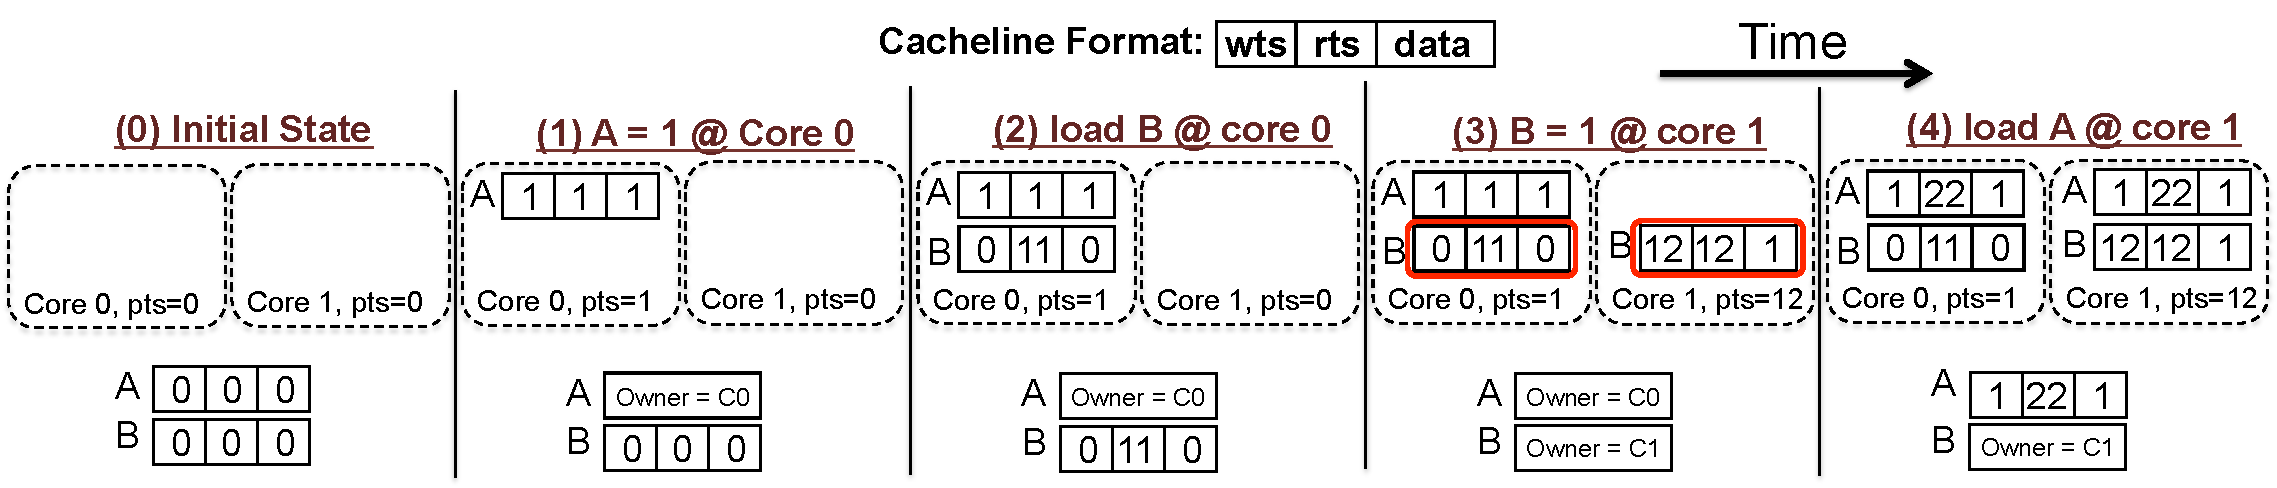
\includegraphics[width=0.95\columnwidth]{figs/example.pdf}
	\caption{ Tardis example program.}
	\label{fig:example}
\end{figure}

\begin{enumerate}
\setcounter{enumi}{-1}
	
\item The initial state of the two cores and two cachelines in the LLC

\item Core 0 writes cacheline A and the LLC registers that it is 
exclusively owned by core 0. PTS in core 0 is increased to 1 because 
an action, in this case changing its value to 1, is performed and thus 
it is advancing in logical time.  

\item Core 0 reads cacheline B. PTS of core 0 remains 1 because 
although cacheline B was loaded, no update was performed on it. B is 
only being read, so its RTS increases to PTS + 10 = 11, where 10 is an 
arbitrarily picked lease value, to indicate a period of validity that 
lasts until PTS exceeds 11. Methods of choosing lease will be 
discussed in the optimizations section. In the LLC, B’s timestamps are 
changed to reflect that it is being leased.

\item Core 1 write cacheline B, but B is currently being read by core 
0, so when it puts B in the exclusive state, PTS, RTS, and WTS are all 
set to 11 + 1 = 12 to depict that core 1 is logically ahead of core 0.  
B’s timestamps show that the Bs in each core are existing at different 
places in logical time which means it having value of 0 in core 0 and 
a value of 1 in core 1 is perfectly valid.  This is the phenomenon of 
``traveling in time'' that is unique to Tardis because cacheline B is 
existing in different logical times at the same instant in physical 
time.  

\item Core 1 now needs to read A, so it leases the cacheline for 10 
timestamps, which makes its RTS = 12 + 10 = 22 where 12 is the PTS of 
core 1 and 10 is the arbitrarily chosen lease. Since it is now being 
read and not edited, its exclusive ownership by core 0 changes to 
shared ownership, as reflected in the timestamps in the LLC.
\end{enumerate}

\section{Optimizations} \label{sec:optimization}

In this section, we will detail the three optimizations we have 
implemented to improve the efficiency and storage overhead of Tardis.

\subsection{Timestamp Compression}

One of the major structural changes implemented in Tardis is the 
inclusion of two timestamps in each cacheline. This translates to a 
large additional requirement for memory, so the optimization of 
timestamp compression was researched to reduce storage costs. We 
exploit the fact that the two timestamps of each cacheline are usually 
fairly close, so we implement a base timestamp (BTS) and a two deltas 
that represent RTS $-$ BTS and WTS $-$ BTS respectively. These two 
deltas are used in place of the actual RTS and WTS timestamps for 
cachelines in a cache, and one 64 bit BTS exists per core. The real 
RTS and WTS values can be calculated by adding each respective delta 
to the BTS which allows the sizes of the deltas to be much smaller 
than their precursor timestamps. The timestamps were originally 64 
bits each, so two timestamps per 512 bits of data is a 25\% storage 
overhead, and not efficient.  With the BTS and deltas, we were able to 
dramatically reduce storage costs. 

We also encountered the problem with timestamp rollover, where a 
timestamp would numerically increase beyond what BTS + delta could 
numerically support. When this happened, all deltas are decreased by 
half the maximum delta value and the BTS is increased by the same 
amount. This calculation is known as rebasing and preserves numerical 
values while freeing up room for the deltas to continue increasing.  
There will probably be some cachelines whose deltas become negative 
after this calculation. In that case, if the cacheline is in the 
exclusive state, its deltas are set to zero because the core its in is the 
only one with claim over the data and doing so will not affect other 
cores. If the cacheline is shared, then the cacheline is invalidated 
and a renew request is sent to the LLC. 

\subsection{Livelock Detection} \label{sec:livelock-detection}

\begin{center}
	
	\begin{tabular}{p{5cm} p{5cm}}
		\textbf{Core 0} & \textbf{Core 1} \\
		\begin{algorithm}[H]
			\While{!done}
			{(nothing)}
			
		\end{algorithm}
		&
		\begin{algorithm}[H]
			$done$ = false $\rightarrow$  true
		\end{algorithm}
		\\
	\end{tabular}
	
\end{center}

The problem with livelock occurs when a core needs to wait for one or 
more cachelines to satisfy certain parameters before continuing 
forward. However, those cachelines never change because PTS does not 
increase since the core’s processes are not going forward in the first 
place. Take  the example above. Core 0 is waiting for \textit{done} to 
be true before continuing via an empty while loop. Core 0 will never 
realize that \textit{done} becomes true because an empty loop will not increase 
the core's PTS. When a core behaves like this, it is known as 
"spinning" because the core constantly monitors, or ``spins", on a 
variable. We optimized the solution to this problem. 

%\begin{enumerate}
The baseline solution was to increment the PTS after a constant number 
of core cycles. This simple solution worked because a constantly 
increasing PTS meant that every cacheline would expire eventually and 
be updated from the LLC. The variable causing the spinning is updated 
and allows the core to move out of livelock. However, this method did 
not seem like the most effective solution because there could still be 
a relatively long time from when the spinning variable changes in the 
LLC to when the version of the variable within the core expires.  
Within this time period the core is spinning, thus doing nothing, and 
our goal was to minimize this gap. 
	
	\begin{comment}
	\item        Implement a “livelock bit” in the core, a livelock counter in the core, and an access counter in each cacheline. This is a two-step process that first checks whether there is a livelock, and then renews the cachelines that seem to be causing the livelock. This scheme is invoked every memory access. By using variable last\_cts, the core is able to determine whether the PTS has increased since the last memory access. If it did increase, then that means the core is progressing that there is no livelock. If the PTS did not change, then the livelock counter is incremented by 1. When it reaches a certain livelock threshold value, the livelock bit, initially false, is set to true to signal that there is a livelock going on. Henceforth, whenever a cacheline is accessed, its individual access counter is incremented by one until it reaches an access threshold, in which case that specific cacheline is renewed. At any time during this process, if the PTS changes when compared to last\_cts, then all counters are reset to 0 and the livelock bit is set to false.
	\end{comment}
	
Our optimization aims to target specific cachelines that could be 
causing the livelock. This approach will reduce the network traffic 
overhead when compared to the original scheme by only sending renew 
requests for a few possibly spinning cachelines.
	
This optimization was incorporated by using a cacheline buffer in 
addition to self increment. The buffer keeps tracks of the last eight 
cachelines accessed, and each cacheline is given with a counter with 
the initial value of 0. When a cacheline in the buffer is accessed 
again, the counter increments. When the counter hits the threshold of 
100 accesses, a check request message is sent to the LLC to see if the data is 
still valid.
    
In the event of a livelock, the counters for the variables responsible
for the spinning will increase to 100 very fast and the livelock can	
be resolved with the check request. If there is no livelock, then the 
core will be accessing different addresses and since the buffer only 
keeps track of last cachelines accessed, no counter will reach 100 and 
no check requests will be sent.
%	[Need test results]
%\end{enumerate}

\subsection{Lease Prediction} \label{sec:lease-prediction}
\begin{center}

\begin{tabular}{p{5cm} p{5cm}}
	\textbf{Core 0} & \textbf{Core 1} \\
	\begin{algorithm}[H]
		\While{true}{
			read A\;
			B++\;
		}

\end{algorithm}
&
\begin{algorithm}[H]
		\While{true}{
			read A\;
			B++\;
		}
\end{algorithm}
\\
\end{tabular}

\end{center}

One of the major issues with Tardis is the fact that because of the 
concept of a lease, timestamps, specifically the PTS, will increase 
rapidly if a cacheline is write-intensive. Consider the example above.  
Assume the lease is arbitrarily chosen as 10. Since B is 
write-intensive, many renew requests for exclusive ownership will be 
made to maintain coherence between the two cores, thus causing the PTS 
to increment quickly in steps of 10. Therefore, although A is 
read-only, the cacheline needs to be repetitively renewed 
unnecessarily, as its lease constantly expires. Since renew requests 
incur extra latency and network traffic, this primitive static lease 
protocol is undesirable. Further motivating the need for a better 
lease protocol can be seen in \ref{fig:renewals}. For certain 
benchmarks, about 60\% of requests are renews, while a significantly 
small percentage of renewal requests are miss speculations, which are 
necessary renews.

\begin{figure}
\begin{center}
  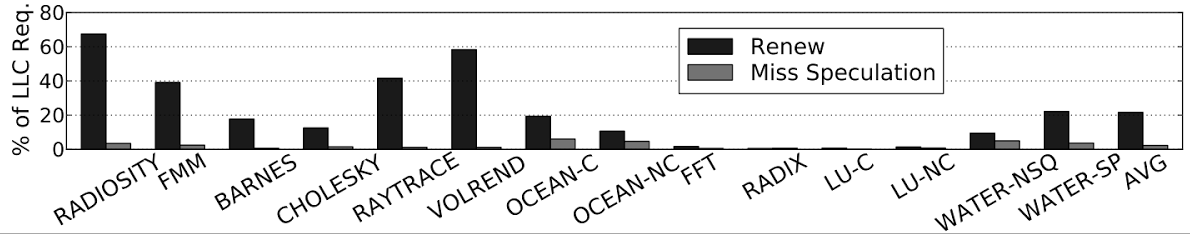
\includegraphics[width=16cm]{image1.png}
  \caption{Graph illustrating the percentage of renew requests and miss speculations (requests that actually necessary) for various benchmarks. }
  \label{fig:renewals}
\end{center}
\end{figure}

With these observations in mind, we notice that write-intensive lines 
should have very small lease sizes so that when renew requests are 
sent, we prevent prolific increase in timestamps. On the other hand, 
since renewing is unnecessary in read-only lines, there is a potential 
for much larger leases. The basic implementation idea is that if data
is renewed, then we progressively give the cacheline a larger lease 
whereas data that are suspected to be read-only are incrementally 
given longer leases, for later renewals. In order to maintain these 
lease states, we add an $n$-bit counter to the cacheline that will 
keep track of a particular line’s “state.” Thus, if $n$ is 2, for 
example, four states exist, namely 00, 01, 10, and 11. 

Since this lease protocol is a very broad idea, we developed 
implementations that require several parameters, or different 
variations. One parameter is the value of $n$. If $n$ is larger, this 
could allow for a more calibrated lease predictor, as the number of 
states increases exponentially, but also creates much more storage 
overhead (extra $n$ bits per cacheline). In this report, we chose $n$ 
to be 2. Another choice is either decrementing the state progressively 
when a line requests exclusive ownership (10 $\rightarrow$ 01) or 
clearing the state counter immediately (10 $\rightarrow$ 00). In 
either case though, if a lease expires, we increment the state from 00 
to 01, for example. We chose to clear the state counter immediately in 
our experiments. The third parameter to be examined is the mapping 
from state to the actual lease. We have two basic algorithms, one is 
an exponentially growing lease and the other is a linearly growing 
one.  Both are similar in nature, and revolve around the same ideas 
previously mentioned, but increase differently, as evident from the 
names. We chose the exponential scheme in this report since this 
scheme gives us larger lease for read only data.

\section{Methodology}

We used the Graphite simulator~\cite{graphite} to model our multicore 
architecture. Graphite is able to simulate 
systems with up to 1000 cores. In this report, we only simulate a 
64-core system, which matches the latest Intel multicore 
processor~\cite{xeonphi}. Each core has a 32~kB private cache and all 
cores share a 8~MB shared cache. All the cores and caches are 
connected using an on-chip network with MESH topology.

\begin{table}
	\caption{ Default Configuration of Tardis. }
	\begin{center}
	{ 
		\begin{tabular}{|l|l|}
            \hline
			\multicolumn{2}{|c|}{Timestamp Compression} \\
			\hline
			Delta timestamp size 		& 20~bits \\
			L1 Rebase Overhead 			& 128~ns\\
			L2 Rebase Overhead			& 1024~ns \\
			\hline
			\multicolumn{2}{|c|}{Livelock Detection} \\
			\hline
			Livelock detection 			& turned on \\
			Self increment period 		& 1000 \\
			\hline
			\multicolumn{2}{|c|}{Lease Prediction} \\
			\hline
			Lease prediction			& turned on \\
			Start lease 				& 8 \\
			Increase factor				& 2 \\
			\hline
		\end{tabular}
    }
	\end{center}
    \label{tab:system}
	\vspace{-.2in}
\end{table}

\cref{tab:system} shows the default configuration of Tardis. All the 
three optimizations introduced in \cref{sec:optimization} are turned 
on by default. The default delta timestamp size is 20~bits. The
rebased overhead for L1 and L2 cache is 128~ns and 1024~ns 
respectively. During this time, the cache is not able to serve other 
requests. The default self increment period is chosen to be 1000. The 
start lease is 8 for each cacheline and the increase factor is 2. 
Unless otherwise stated, all the experiments use these parameters by 
default.

We use a subset of Splash-2~\cite{splash2} benchmarks to evaluate our 
optimization techniques. For each experiment, we show the speedup, or 
throughput (in bars) and the renew rate (in red dots) for each 
benchmark.

\section{Evaluations}

In this section, we evaluate the performance of the optimization 
techniques introduced in \cref{sec:optimization}.

\subsection{Main Result}

\begin{figure}
	\centering
	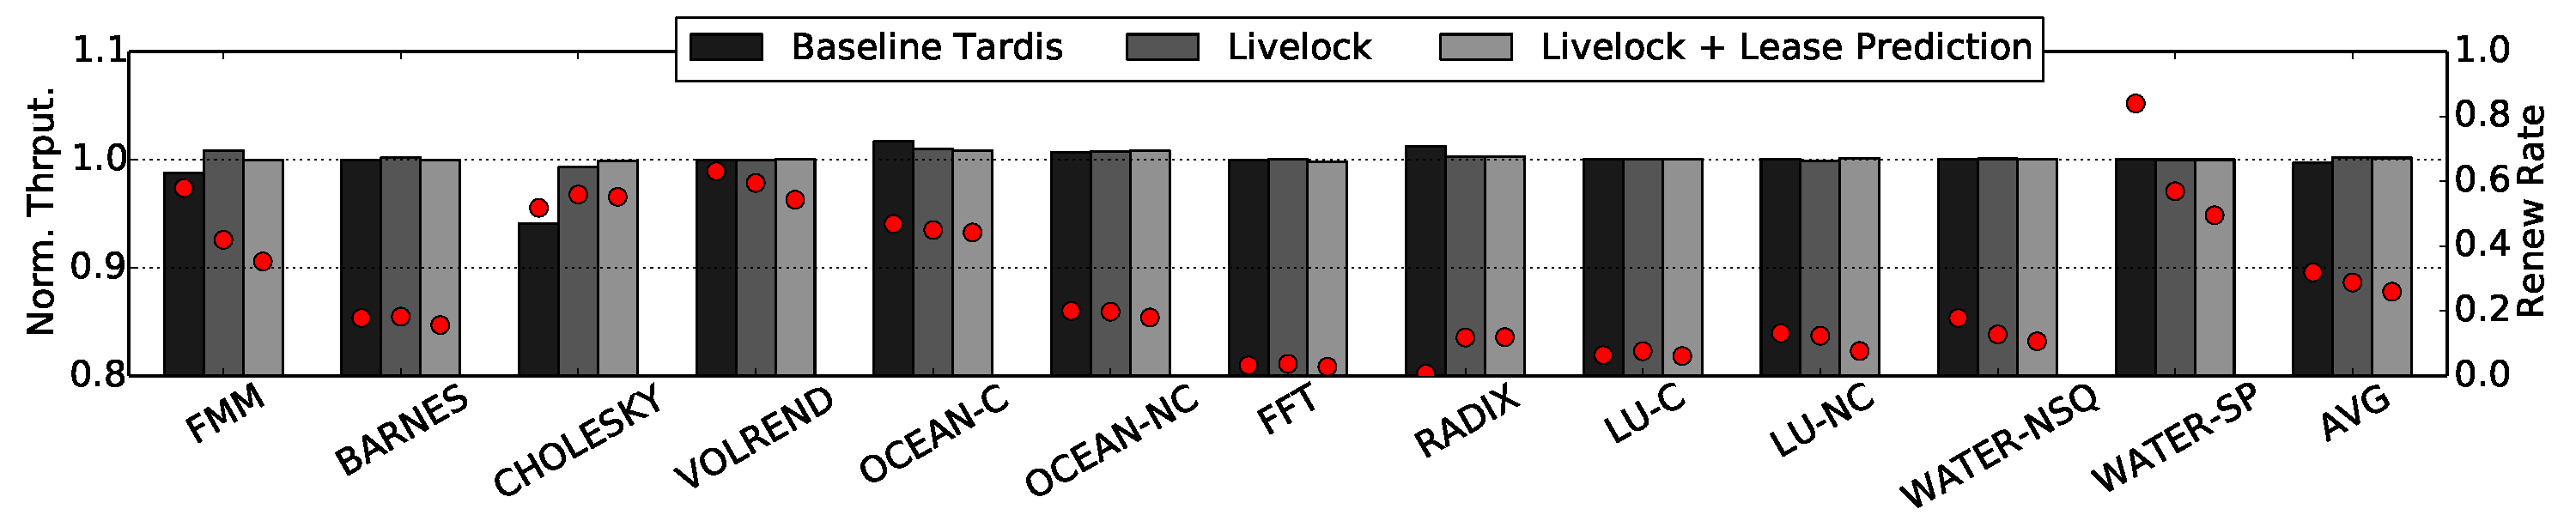
\includegraphics[width=0.95\columnwidth]{figs/main.pdf}
	\caption{ Tardis with different optimization techniques.}
	\label{fig:main}
\end{figure}

\cref{fig:main} summarizes the performance improvement of the 
optimization techniques introduced in this report. Here we show the 
performance of the baseline directory protocol, the baseline Tardis protocol~\cite{tardis}, the baseline Tardis with livelock 
detection (\cref{sec:livelock-detection}) and Tardis with both livelock 
detection and lease prediction (\cref{sec:lease-prediction}).

%\red{TODO}

We note that livelock detection improves performance for benchmarks that heavily using spinning, such as Cholesky and FMM, and that livelock detection and lease prediction used in conjunction reduces the renew rate and network traffic for most benchmarks.

\subsection{Timestamp Compression}

\begin{figure}
	\centering
	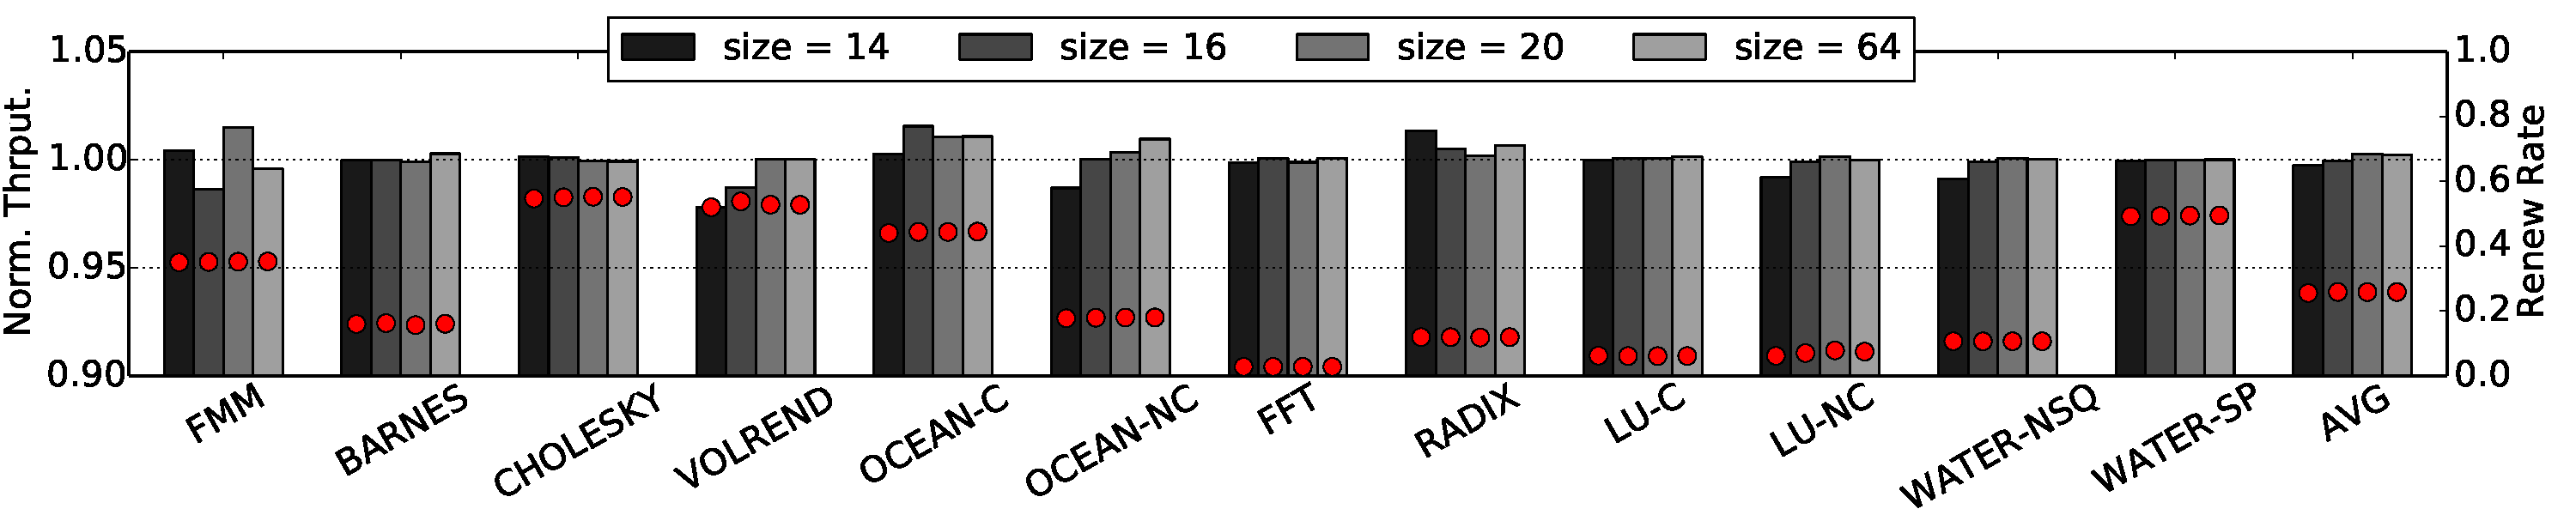
\includegraphics[width=0.95\textwidth]{figs/tssize.pdf}
	\caption{ Performance of Tardis sweeping the delta timestamp size}
	\label{fig:tssize}
\end{figure}

A delta that was too small would mean frequent rebasing and lower 
performance while a delta too large would cause this optimization to 
be ineffective. Through our benchmarking tests with various delta 
sizes, we found a size of 14 bits had bad performance. 16 Bits was 
better, but we chose 20 bits in the end because it was the smallest 
value that had no noticeable impact on performance. \cref{fig:tssize} shows 
that  there is noticeable performance gain when increasing the delta 
size from 14 to 16 to 20, but the difference between 20 bits and 64 
bits is insignificant when considering the large difference in the 
storage size. As long as the delta size is large enough to prevent 
overly frequent rebasing, performance is not sensitive to timestamp 
size, which makes 20 bits our optimal value for the delta timestamp 
size.

\subsection{Livelock Detection}

\begin{figure}
	\centering
	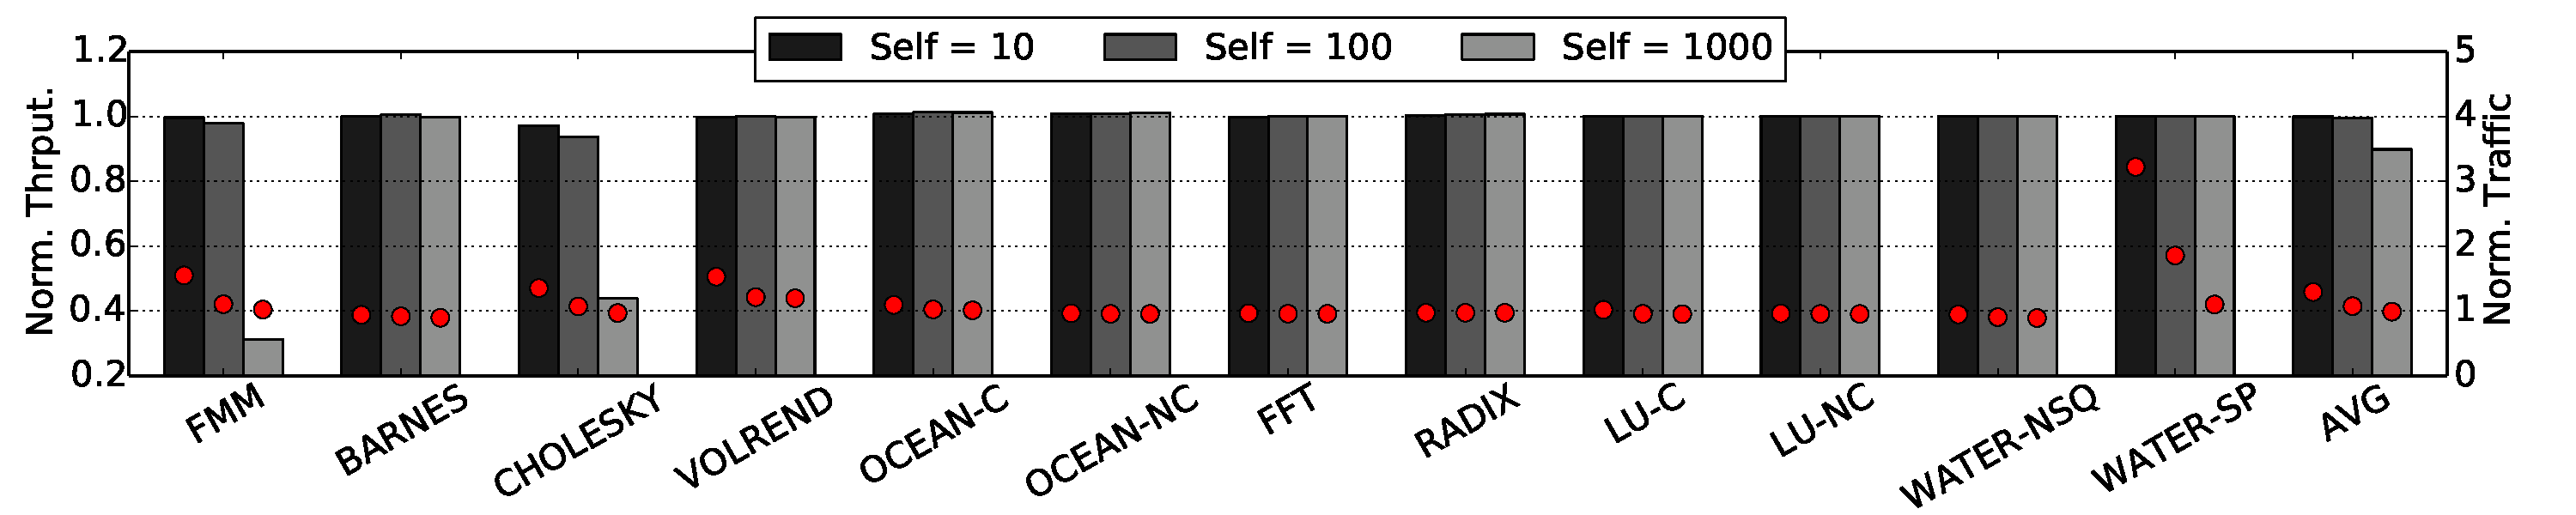
\includegraphics[width=0.95\columnwidth]{figs/selfincr_nolive.pdf}
	\caption{ Baseline Tardis without livelock detection. }
	\label{fig:self-nolive}
\end{figure}

We studied the self increment method by changing the self increment 
period, which is the amount of CPU cycles that the core goes though 
per 1 pts increment. As seen with \cref{fig:self-nolive}, a low self 
increment period resulted in higher network traffic because of 
frequent renew requests while a larger period decreased the renew rate 
but resulted in a lower performance since a livelock took longer to 
resolve.  
  
  
By implementing the livelock detection system, we eliminated the 
decrease in performance while maintaining the gains of lower renewals 
and reduced network traffic~\cref{fig:self-live}.  A larger self 
increment period does not hurt performance anymore because our 
optimization deals with the livelock as soon as it occurs by detecting 
it and renewing the relevant cachelines. The core no longer has to 
wait for self increment for those cachelines to expire and that is 
what results in the lack of performance loss from large self increment 
periods.

\begin{figure}
	\centering
	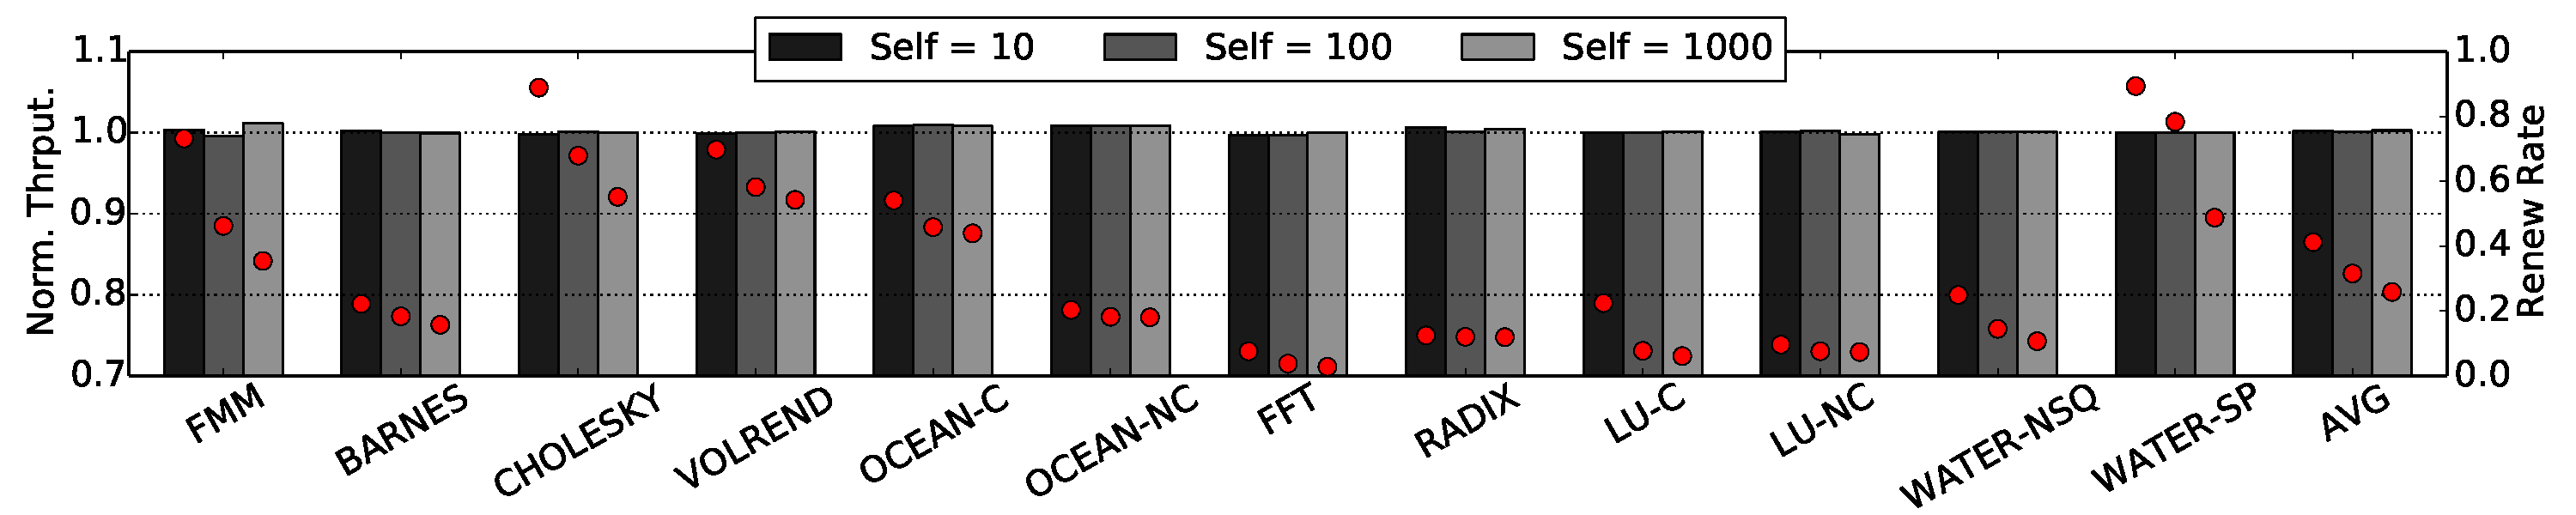
\includegraphics[width=0.95\columnwidth]{figs/selfincr_live.pdf}
	\caption{ Tardis with livelock detection. }
	\label{fig:self-live}
\end{figure}


\subsection{Lease Prediction}

\begin{figure}
	\centering
	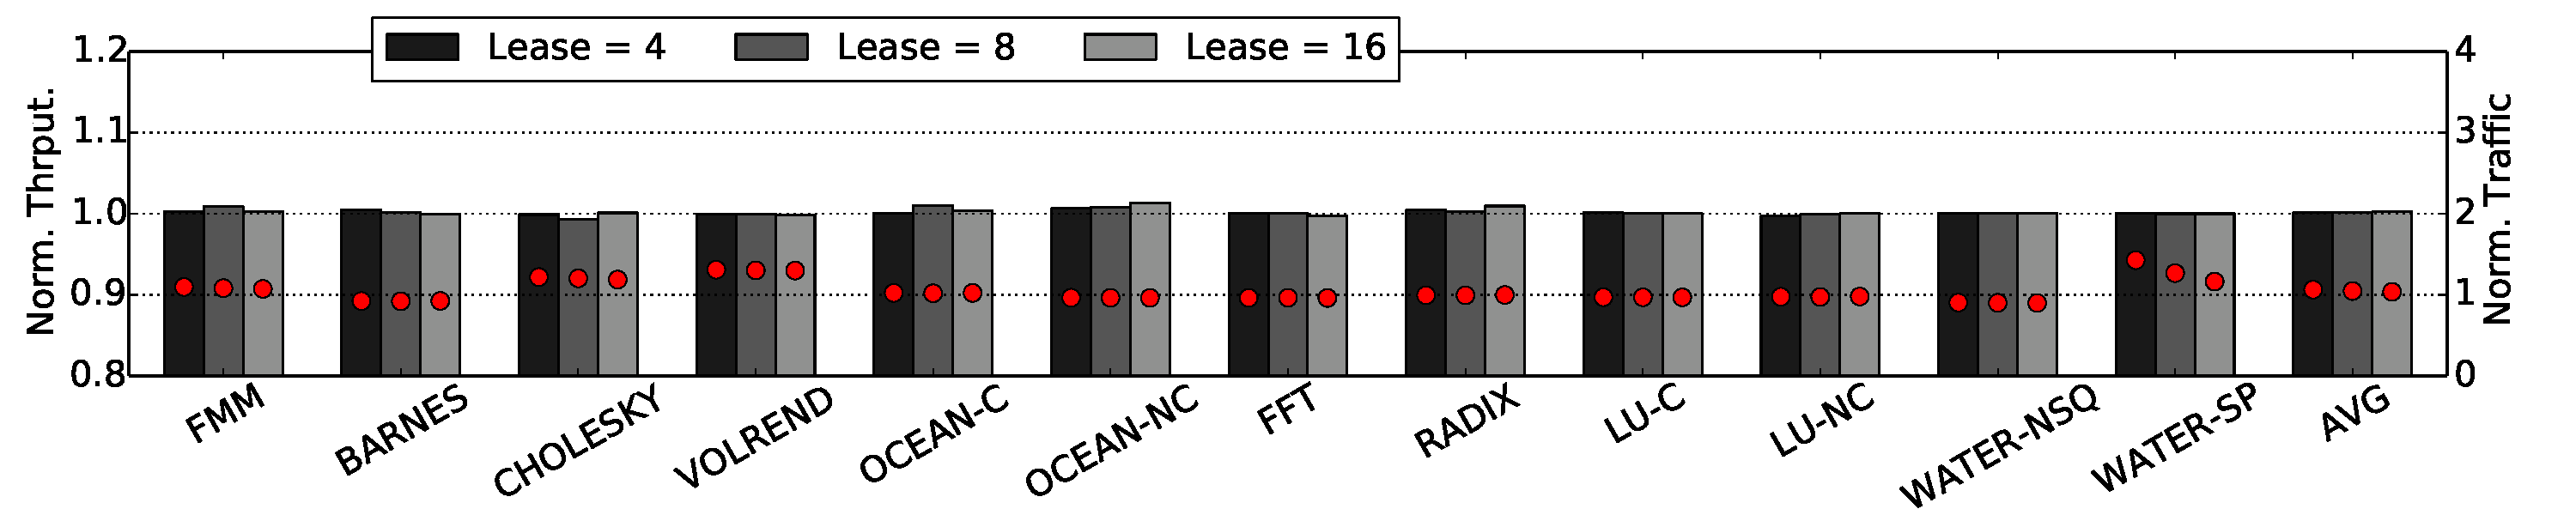
\includegraphics[width=0.95\columnwidth]{figs/static.pdf}
	\caption{ Sweeping the static lease.  }
	\label{fig:static}
\end{figure}

%We did not examine the effect of using three bits for the state size, 
%because 8 possible states with an increase factor of 8 would lead to 
%a lease that is at least $8^8$, over 16 million, an unnecessarily 
%large  lease.

\cref{fig:static} sweeps the static lease from 4 to 16. Livelock 
detection is enabled in this experiment. It is important to note that 
performance is not sensitive to the value of static lease, due to the 
face that we enabled livelock detection. Without livelock detection, 
performance drops with large lease values for benchmarks that heavily 
use spinning variables. Renew rate reduces slightly for most 
benchmarks because of fewer renew requests with larger leases. This is 
most significantly evident in Water-Spatial.

\begin{figure}
	\centering
	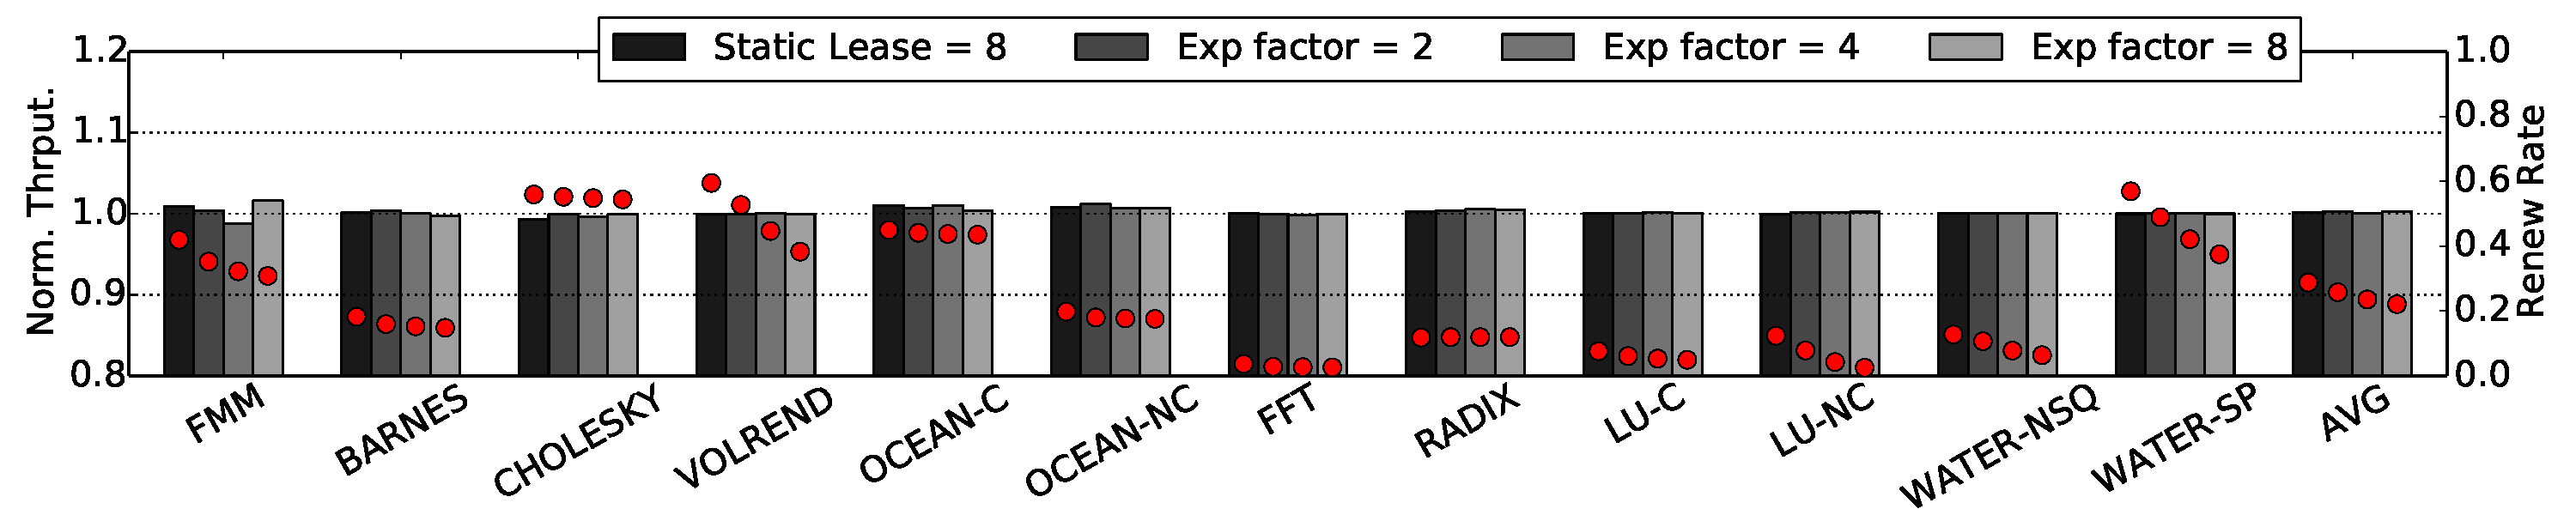
\includegraphics[width=0.95\columnwidth]{figs/exp.pdf}
	\caption{ Sweeping the increase factor for lease prediction 
	algorithm.}
	\label{fig:exp}
\end{figure}

\cref{fig:exp} shows the performance of our exponential lease 
prediction algorithm discussed in \cref{sec:lease-prediction}. We tested the linear prediction method as well, but found exponential to be significantly better performance. Thus, all the experiments are done with an exponential lease.
%[Should we explain why no need to test linear?]
% if you want, we can say that we tested both, and figured that 
% exponential has better performance. 
Here, the lease prediction algorithm does not affect throughput 
because speculation prevents throughput from improving.

Lease prediction does, however, reduce the renewal rate and network 
traffic. The reduction is more significant than simply using a larger 
static lease (\cref{fig:static}) which is apparent in many of the 
benchmarks.

\section{Future Work}

The current lease prediction algorithm is simple, and we believe that 
there may be better protocols to further decrease renewal rate for all 
benchmarks. There is a large design space with lease prediction, so we 
will be exploring new ideas.

Another idea to further improve the performance of Tardis is to 
combine it with another protocol. One such protocol in mind is the 
MESI cache coherence protocol, in which each cacheline is marked with 
one of four states, as opposed to one of three in the MSI directory 
protocol.

\section{Conclusion}

Tardis is a new scheme to ensure memory coherence. Its main advantages 
are its scalability, simplicity, and to perform operations that 
``travel in time'' by using logical time, incorporated with timestamps 
in cachelines and cores. We tested multiple optimizations involving 
timestamp compression, lease prediction, and livelock detection, and 
were successful in improving important drawbacks of Tardis as a whole. Throughput is improved by up to 6\% and renew rate is reduced from 32\% to 26\%.

{
	\bibliographystyle{abbrv}
	\bibliography{refs}
}
\end{document}

